%% -*- coding:utf-8 -*-

%%%%%%%%%%%%%%%%%%%%%%%%%%%%%%%%%%%%%%%%%%%%%%%%%%%%%%%%%
%%   $RCSfile: 5-merkmalstrukturen.tex,v $
%%  $Revision: 1.13 $
%%      $Date: 2010/11/16 08:40:32 $
%%     Author: Stefan Mueller (FU Berlin)
%%    Purpose: 
%%   Language: LaTeX
%%%%%%%%%%%%%%%%%%%%%%%%%%%%%%%%%%%%%%%%%%%%%%%%%%%%%%%%%

\chapter{特征描写}
%\chapter{Feature descriptions}
\label{chap-feature-descriptions}

在上一章,我们谈到了可以用来描写语言对象的特征-值偶对。本章中,我们将介绍在词汇功能语法、中心语驱动的短语结构语法、构式语法、范畴语法、树邻接语法,甚至是最简方案的某些形式化理论\citep{Veenstra98a}中发挥重要作用的特征描写。本章将为后面的章节打下一些基础。
%In the previous chapter, we talked about sets of feature-value pairs, which can be used to describe linguistic objects. In this chapter, we will %introduce
%feature descriptions which play a role in theories such as LFG, HPSG, Construction Grammar, versions of Categorial Grammar and TAG (and %even some
%formalizations of Minimalist theories \citep{Veenstra98a}). This chapter will therefore lay some of the groundwork for the chapters to follow.

特征结构是可以模拟语言对象属性的复杂实体。语言学家们多半只用特征描写来描写特征结构的某些部分。我们将在\ref{sec-modelle-theorien}详细解释模型与描写之间的差异。
%Feature structures are complex entities which can model properties of a linguistic object. 
%Linguists mostly work with feature descriptions which describe only parts of a given feature
%structure. The difference between models and descriptions will be explained
%in more detail in Section~\ref{sec-modelle-theorien}.

表示特征结构的其他术语有:
%Alternative terms for feature structures are:
\begin{itemize}
\item 特征-值结构\isce{特征-值结构}{feature-value structure}
\item 属性-值结构\isce{属性-值结构}{attribute-value structure}
%\item feature-value structure\is{feature-value structure}
%\item attribute-value structure\is{attribute-value structure}
\end{itemize}
其他特征描写的术语有:
%Other terms for feature description are the following:
\begin{itemize}
\item \emph{特征-值矩阵}(AVM)\isce{特征-值矩阵}{attribute-value matrix (AVM)}
\item \emph{特征矩阵}
%\item \emph{attribute-value matrix} (AVM)\is{attribute-value matrix (AVM)}
%\item \emph{feature matrix}
\end{itemize}
接下来,为了保证本书的形式部分尽可能地简短,我将只讨论必要的细节。我推荐感兴趣的读者参考 \citet{Shieber86a}、 \citet[\S~2]{ps}、 \citet{Johnson88}、 \citet{Carpenter92a}、 \citet{King94a}和 \citet{Richter2004a-u}。Shieber的著作对合一语法的介绍浅显易懂。King和Richter介绍了HPSG的重要理论基础,这对于在数学方面没有打下良好基础的读者来说是较为容易理解的。尽管如此,知道这些文献的存在,并且了解相应理论建立的基础是非常重要的。
%In what follows, I will restrict the discussion to the absolutely necessary details in order to keep the formal part of the book as short as %possible. I refer
%the interested reader to  \citet{Shieber86a},  \citet[Chapter~2]{ps},  \citet{Johnson88},  \citet{Carpenter92a},
% \citet{King94a} and  \citet{Richter2004a-u}. Shieber's book is an accessible introduction to Unification Grammars. The works by King and %Richter, which introduce important
%foundations for HPSG, would most probably not be accessible for those without a good grounding in mathematics. 
%However, it is important to know that these works exist and that the corresponding linguistic theory is build on a solid foundation.

\section{特征描写}
%\section{Feature descriptions}

在\isce[|(]{特征描写}{feature description}描写语言符号时,我们必须要对它们的属性进行说明。对于名词而言,它们有格、性、数和人称的特征。以“男人”这个词为例,属性特征的取值为“属格”、“阳性”、“单数”和“第三人称”。如果我们要将这些信息写成一个特征-值偶对的列表的话,我们就会得到下面的特征描写:
%When\is{feature description|(} describing linguistic signs, we have to say something about their properties. For a noun, we can say that it has %case, gender, number and person features.
%For a word such as  \emph{Mannes} `man', we can say that these features have the values \emph{genitive}, \emph{masculine}, %\emph{singular} and \emph{3}.
%If we were to write these as a list of feature-value pairs, we would arrive at the following feature description:
\eas
“男人”的特征-值偶对:\\
%Feature-value pair for \emph{Mannes}:\\
\ms{
%格   & 属格\\
%性   & 阳性\\
%数 & 单数\\
%人称   & 第3人称\\
格   & 属格\\
性   & 阳性\\
数 & 单数\\
人称  & 第3人称\\
}
\zs
我们也可以用特征描写来描述不同的事物。例如,我们可以像例(\mex{1})那样来描写一个人:
%It is possible to describe a variety of different things using feature descriptions. For example, we can describe a person as in (\mex{1}):
\ea
\ms{
%名    & max\\
%姓   & meier\\
%出生日期 & \zhdate{1985/10/10}\\
名    & max\\
姓   & meier\\
出生日期  & \normalfont\zhdate{1985/10/10}\\
}
\z
人与人之间的关系也可以在特征-值偶对中表示。例如,Max Meier的父亲叫做Peter Meier这样的事实可以通过对(\mex{0})的扩展来表示,如下所示:
%People are related to other people -- a fact that can also be expressed in feature-value pairs. For example, the fact that Max Meier has a %father
%called Peter Meier can be captured by expanding (\mex{0}) as follows: 
\ea
\ms{
名    & max\\
姓    & meier\\
出生日期  & \normalfont\zhdate{1985/10/10}\\
父亲     & \ms{
             名 & peter\\
             姓   & meier\\
             出生日期    & \normalfont\zhdate{1960/05/10}\\
             父亲     & \ldots\\
             母亲   & \ldots\\
             }\\
母亲		 & \ldots\\
}
\z
“\textsc{父亲}”特征的值是包含(\mex{-1})中同样特征的特征描写。
%The value of the \textsc{父亲} feature is another feature description containing the same features as (\mex{-1}).

在特征描写中,路径(path)\isce{路径}{path}是指一个接一个的特征的序列。路径值(value of a path)是在路径末端的特征描写。由此,“\textsc{父亲$|$出生日期}”的值为“\zhdate{1960/05/10}”。
%In feature descriptions, a \emph{path}\is{path} is a sequence of features which immediately follow each other.
%The \emph{value of a path} is the feature description at the end of the path. Therefore,
%the value of \textsc{father$|$出生日期 } is \emph{10.05.1960}.

我们可以想到,像(\mex{0})这样的表示中可以囊括许多不同的特征。有人可能会问,如何在(\mex{0})中加入后代的信息呢?
%One can think of many different features that could be included in representations such as (\mex{0}). One may wonder how
%to integrate information about offspring into (\mex{0}).

一个显而易见的解决方案就是加入“\textsc{女儿}”和“\textsc{儿子}”这两个特征:
%An obvious solution would be to add features for \textsc{daughter} und \textsc{son}:
\ea
\ms{
名    & max\\
姓   & meier\\
出生日期  & \normalfont\zhdate{1985/10/10}\\
父亲      & \ldots\\
母亲     & \ldots\\
女儿    & \ldots\\   
}
\z
但是,这个方法也有让人不满意的地方,比如它无法直接清晰地说明如何来描写有几个女儿的人。是否应该引入诸如“\textsc{女儿-1}”或“\textsc{女儿-3}”这样的特征呢?
%This solution is not satisfactory as it is not immediately clear how one could describe a person with several daughters.
%Should one really introduce features such as \textsc{daughter-1} or \textsc{daughter-3}?
\ea
\ms{
名      & max\\
姓      & meier\\
出生日期 & \normalfont\zhdate{1985/10/10}\\
父亲    & \ldots\\
母亲    & \ldots\\
女儿-1  & \ldots\\   
女儿-2  & \ldots\\
女儿-3  & \ldots\\
}
\z
我们想要设定多少个特征呢?数量的限制是多少?“\textsc{女儿-32}”的值会是什么呢?
%How many features do we want to assume? Where is the limit?
%What would the value of \textsc{daughter-32} be?

就此例而言,用列表\isce{列表}{list}更为合理。列表用尖括号表示。任意数量的元素可以出现在这些尖括号中。特殊的情况是,在这些括号中并没有元素。一个没有元素的列表被叫做空列表(empty list)。下例中,Max Meier有一个女儿叫做Clara,而她没有女儿。
%For this case, it makes much more sense to use a list\is{list}. Lists are indicated with angle brackets. Any number of elements can occur %between
%these brackets. A special case is when no element occurs between the brackets. A list with no
%elements is also called \emph{empty list}. In the following example,
%Max Meier has a daughter called Clara, who herself has no daughter.
\ea
\ms{
名    & max\\
姓    & meier\\
出生日期  & \normalfont\zhdate{1985/10/10}\\
父亲      & \ldots\\
母亲     & \ldots\\
女儿    & \liste{ \ms{
                     名    & clara\\
                     姓    & meier\\
                     出生日期  & \normalfont\zhdate{2004/10/10}\\
                     父亲      & \ldots\\
                     母亲     & \ldots\\
                     女儿   & \liste{ }\\   
} }\\   
}
\z
现在,我们还剩下与儿子有关的问题。是否应该加上一个儿子的列表?我们希望区分儿子和女儿吗?显然,孩子的性别是一个重要的属性,这些是客体本身的属性,因为每个人都有性别。由此,(\mex{1})中的描写更为合适。
%Now, we are left with the question of sons. Should we add another list for sons? Do we want to differentiate between sons and daughters?
%It is certainly the case that the gender of the children is an important property, but these are
%properties of the objects themselves, since every person has a gender. The description in (\mex{1}) therefore offers a more adequate %representation.

%\begin{figure}[tb]
\ea
\ms{
名    & max\\
姓    & meier\\
出生日期  & \normalfont\zhdate{1985/10/10}\\
\textbf{性别} & \textbf{男}\\
父亲      & \ldots\\
母亲     & \ldots\\
子女    & \liste{ \ms{
                     名    & clara\\
                     姓    & meier\\
                     出生日期  & \normalfont\zhdate{2004/10/10}\\
                     \textbf{性别} & \textbf{女}\\
                     父亲      & \ldots\\
                     母亲     & \ldots\\
                     子女     & \liste{ }\\   
} }\\   
}
\z
%\vspace{-\baselineskip}
%\end{figure}%
到这儿,有人可能会问为什么父母没有用列表表示。事实上,我们在语言学的研究中也发现了类似的问题:如何针对现在的任务来对信息进行最有效的表示?有人可能会提出用单独的特征来表示父母的描写,并指出这样的表示可以对母亲或者父亲进行一定的说明,而不用在列表中检索他们各自的描写。
%At this point, one could ask why the parents are not included in a list as well. In fact, we find similar questions also
%in linguistic works: how is information best organized for the job at hand? One could argue for the
%representation of descriptions of the parents under separate features, by pointing out that with
%such a representation it is possible to make certain claims about a mother or father without having to necessarily
%search for the respective descriptions in a list.

如果元素的序列是无关的,那么我们可以用集合\isce{集合}{set},而不是列表。集合用弧形括号(curly brackets)表示。\footnote{%
集合的定义需要很多技术指标。本书中,我只用集合来表示语义信息。这点用列表也可以做到,这就是为什么我在这里没有引入集合,而是使用了列表。
}
%If the order of the elements is irrelevant, then we could use sets\is{set} rather than lists.
%Sets are written inside curly brackets.\footnote{%
%The definition of a set requires many technicalities. 
%In this book, I would use sets only for collecting semantic information. This can be done equally
%well using lists, which is why I do not introduce sets here and instead use lists.%
%}

\section{类型}
%\section{Types}
\label{sec-formalismus-typen}

在\isce[|(]{类型}{type}上一节,我们介绍了包括特征-值偶对的特征描写,并且说明了应该允许特征被赋予复杂的值。在本节,特征描写将扩大到包括类型。赋予了类型的特征描写也叫做类型特征描写。类型说的是哪些特征可以或者必须属于一个具体的结构。前面讲到的描写是关于属于类型“\type{人}”的某一客体的。
%In\is{type|(} the previous section, we introduced feature descriptions consisting of feature-value pairs and showed that it makes sense to %allow for
%complex values for features. In this section, feature descriptions will be augmented to include types. Feature descriptions which are assigned %a type
%are also called \emph{typed feature descriptions}. Types say something about which features can or must belong to a 
%particular structure. The description previously discussed describes an object of the type \type{person}.
\ea
\ms[人]{
名    & max\\
姓    & meier\\
出生日期  & \normalfont\zhdate{1985/10/10}\\
性别 & 男\\
父亲      & \ldots\\
母亲     & \ldots\\
子女     & \liste{ \ldots, \ldots{} }
}
\z
%类型用斜体表示。
%Types are written in \textit{italics}. 

类型的具体要求确定了所模拟对象具有的属性。这样,一个理论才能描写这些属性。诸如“\textsc{工作电压}”这样的属性与类型“\textit{人}”是无关的。如果我们知道一个给定对象的类型,那么我们也会知道该对象一定具有某些属性,即使我们还不知道这些属性具体的值。这样,(\mex{1})仍是对Max Meier的描写,即使它并不包含任何有关Max的生日信息:
%The specification of a type determines which properties a modelled object has. It is then only
%possible for a theory to say something about these properties.
%Properties such as \textsc{operating voltage} are not relevant for objects of the type \textit{person}. If we know the type of a given object, then %we
%also know that this object must have certain properties even if we do not yet know their exact values. In this way, (\mex{1}) is still a description %of
%Max Meier even though it does not contain any information about Max' date of birth:
\ea
\ms[人]{
名   & max\\
姓    & meier\\
性别 & 男
}
\z
但是,我们知道Max Meier一定是在某天出生的,因为这是对类型“\textit{人}”的描写。对于(\mex{0})这类结构来说,“Max的生日是什么?”这个问题是有意义的,而“Max有哪种工作电压?”这个问题就是无意义的。如果我们知道某个对象是属于类型“\textit{人}”的,那么就会有如下的基本结构:
%We know, however, that Max Meier must have been born on some day since this is a description of the type \textit{person}.
%The question \emph{What is Max' date of birth?} makes sense for a structure such as (\mex{0}) in a way that the question
%\emph{Which operating voltage does Max have?} does not. If we know that an object is of the type \textit{person}, then we have
%the following basic structure:
\ea
\ms[人]{
名    & 名\\
姓  & 姓 \\
出生日期  & 日期\\
性别 & 性别\\
父亲      & 人\\
母亲    & 人\\
子女    & 人的列表~
}
\z
在(\mex{0})和(\mex{-1})中,“\textsc{名}”这类特征的值也是类型。
%在(\mex{0})和(\mex{-1})中,\textsc{名}这类特征的值用斜体表示。这些值也是类型。
但是,他们与“\type{人}”这类特征不同,因为它们没有次类特征。这些特征叫做“原子式”(atomic)\iscesub{类型}{type}{原子式}{atomic}。
%In (\mex{0}) and (\mex{-1}), the values of features such as \textsc{名} are in italics. These values are also types. They are different from
%types such as \type{person}, however, as no features belong to them. These kinds of types are called \emph{atomic}\is{type!atomic}.

特征按照层级来进行组织\isce[|(]{类型层级体系}{type hierarchy}。
%Types are organized into hierarchies\is{type hierarchy|(}.
对于“\textit{人}”来说,可以界定次类型“\textit{女人}”和“\textit{男人}”。这将测定出给定对象的性别。(\mex{1})显示了类型“\textit{女人}”的特征结构,这与类型“\textit{男人}”的特征结构是相似的。
%It is possible to define the subtypes  \textit{woman} and \textit{man} for  \textit{person}. These would determine the gender of a given object.
%(\mex{1}) shows the feature structure for the type \textit{woman}, which is analogous to that of \textit{man}.
\ea
\ms[女性]{
名    & 名\\
姓  & 姓 \\
出生日期  & 日期\\
性别  & 女\\
父亲      & 人\\
母亲    & 人\\
子女    & 人的列表~   
}
\z
在这点上,我们应该自问是否真的需要“\textsc{性别}”这个特征,因为必要信息已经在“\type{女人}”这个类型中显示出来了。
下面两个问题会在语言分析的讨论中重现:特定的信息是由特定的特征表示的?还是仅存储在一个没有相应的独立特征的类型中?
这两种可选方案的差异主要体现为通过类型模拟的信息的事实没有直接通过结构共享而获得。这点在\ref{sec-strukturteilung}中有所讨论。
%At this point, we could ask ourselves if we really need the feature \textsc{gender}. The necessary information is already represented in the %type \type{woman}.
%The question if specific information is represented by special features or whether it is stored in a type without a corresponding individual %feature will
%surface again in the discussion of linguistic analyses.
%Both alternatives differ mostly in the fact that the information which is modelled by types is not
%immediately accessible for structure sharing, which is discussed in Section~\ref{sec-strukturteilung}.

类型层级体系\label{Seite-Typhierarchie}在捕捉语言学的一般性特征方面发挥了重要的作用,这就是为什么类型层级体系和约束与信息的承继需要在后面的例子中进行解释。我们可以将类型层级体系看成是一种有效的组织信息的方式。在百科辞典中,个体之间是相互联系的,比如说猴子和老师这两个词条的联系在于二者都指向哺乳动物。针对哺乳动物的描写同样也适用于从属于它的概念中。同样,如果我们想要描写不同的电子设备,我们可以应用图\vref{fig-electric-appliance}中的层级体系。
%Type hierarchies\label{Seite-Typhierarchie} play an important role in capturing linguistic generalizations, which is why type hierarchies and
%the inheritance of constraints and information will be explained with reference to a further example in what follows. One can think of type %hierarchies as an effective
%way of organizing information. In an encyclopedia, the individual entries are linked in such a way
%that the entries for monkey and mouse will each contain a pointer to mammal. The description found
%under mammal does therefore not have to be repeated for the subordinate concepts. In the same way,
%if one wishes to describe various electric appliances, one can use the hierarchy in Figure~\vref{fig-electric-appliance}.
\begin{figure}
\centering
%% \begin{forest}
%% typehierarchy
%% [\type{electric appliance}
%%   [\type{printing device}
%%     [\type{printer}
%%       [\type{laser printer}]
%%       [\ldots]]
%%     [\subnode{copier}{\type{photocopier}}] ]
%%   [\subnode{scanning}{\type{scanning device}}
%%     [\type{scanner}
%%       [\type{negative scanner}]
%%       [\ldots] ] ]
%%   [\ldots]]
%% \draw (scanning.south)--(copier.north);
%% \end{forest}
\begin{tabular}{cccc}
\multicolumn{4}{c}{\mynode{ed}{\type{电子设备}}}\\[6ex]
\mynode{p}{\type{打印设备}} & & \mynode{sc}{\type{扫描设备}} & \mynode{other}{\rule[-0.5ex]{0cm}{2.5ex}\ldots}\\[6ex]
\mynode{printer}{\type{打印机}}   & \mynode{copy}{\type{复印机}}  & \mynode{scanner}{\type{扫描机}}\\[6ex]
\mynode{l-p}{\type{激光打印机}}  & \mynode{other-p}{\rule[-0.5ex]{0cm}{2.5ex}\ldots}  & \mynode{negscan}{\type{底片扫描机}} & 
%\multicolumn{4}{c}{\mynode{ed}{\type{electric appliance}}}\\[6ex]
%\mynode{p}{\type{printing device}} & & \mynode{sc}{\type{scanning device}} & \mynode{other}{\rule[-0.5ex]{0cm}{2.5ex}\ldots}\\[6ex]
%\mynode{printer}{\type{printer}}   & \mynode{copy}{\type{photocopier}}  & \mynode{scanner}{\type{scanner}}\\[6ex]
%\mynode{l-p}{\type{laser printer}}  & \mynode{other-p}{\rule[-0.5ex]{0cm}{2.5ex}\ldots}  & \mynode{negscan}{\type{negative scanner}} & 
\mynode{other-sc}{\rule[-0.5ex]{0cm}{2.5ex}\ldots}\\
\end{tabular}
\begin{tikzpicture}[overlay,remember picture,shorten <=2pt,shorten >=2pt] 
\draw(ed.south)--(p.north)
     (ed.south)--(sc.north)
     (ed.south)--(other.north)
     (p.south)--(copy.north)
     (p.south)--(printer.north)
     (printer.south)--(l-p.north)
     (printer.south)--(other-p.north)
     (sc.south)--(copy.north)
     (sc.south)--(scanner.north)
     (scanner.south)--(negscan.north)
     (scanner.south)--(other-sc.north);
\end{tikzpicture}
\caption{\label{fig-electric-appliance}多重承继的非语言学例子}
%\caption{\label{fig-electric-appliance}Non-linguistic example of multiple inheritance}
\end{figure}%
图中最高点是最为普遍的类型“电子设备”(electrical device)。电子设备具有一定的属性,比如说带有特定能量消耗的能量供给。“电子设备”的所有次类型都“承继”了这一属性。这样,“打印设备”和“扫描设备”也具有可供特定能量消耗的能力供给。“打印设备”可以制造信息,而“扫描设备”可以阅读信息。“复印机”既可以制造信息也可以阅读信息。复印机具有扫描机和打印机的属性。这在图\ref{fig-electric-appliance}中通过两个上位类型和“复印机”之间的联系来表示。如果一个类型同时也是几个上位类型的次类型,那么我们就可以说这是多重承继(multiple inheritance)\iscesub{承继}{inheritance}{多重}{multiple}。如果设备可以打印,但是不能扫描,它们就属于类型打印机(printer)。该类型有更多特定的次类型,相应地可具有特殊的属性,比如说“激光打印机”。新的特征可以被加进次类型中,但是也可以将承继的特征的值做得更具体。比如说,可以用“底片扫描机”扫描的材料比它的上位类型“扫描机”具有更多的限制,因为底片扫描机只能扫描底片。
%The most general type \type{electrical device} is the highest in Figure~\ref{fig-electric-appliance}. Electrical devices have certain properties, 
%\eg 
%a power supply with a certain power consumption. All subtypes of  \type{electrical device} ``inherit'' this property. In this way, \type{printing %device} and
%\type{scanning device} also have a power supply with a specific power consumption. A
%\type{printing device} can produce information and a \type{scanning device} can read in information. A \type{photocopier} can both produce %information and read it. Photocopiers have both the properties of scanning and printing devices.
%This is expressed by the connection between the two superordinate types and \type{photocopier} in
%Figure~\ref{fig-electric-appliance}. If a type is at the same time the subtype of several superordinate types, then we
%speak of \emph{multiple inheritance}\is{inheritance!multiple}. If devices can print, but not scan, they are of type \emph{printer}. This type can %have further more
%specific subtypes, which in turn may have particular properties, \eg \type{laser printer}. New
%features can be added to subtypes, but it is also possible to make values of inherited features more
%specific. For example, the material that can be scanned with a \type{negative scanner} is far more
%restricted than that of the supertype \type{scanner}, since negative scanners can only scan negatives.

模拟的对象总是有一个最为具体的类型。在上例中,这意味着可以有类型为“激光打印机”和“底片打印机”的对象,但是没有类型为“打印设备”的对象。这是因为,“打印设备”不是最具体的,该类型有两个次类型。
%The objects that are modeled always have a maximally specific type. In the example above, this means that we can have objects of the type %\type{laser printer} and \type{negative scanner}
%but not of the type \type{printing device}. This is due to the fact that \type{printing device} is not maximally specific since this type has two %subtypes.

带有多重承继的类型层级体系是表达语言概括的重要手段。在这些层级的最高点出现的词或短语的类型对应于语言对象的约束条件,这对于所有语言中的语言对象来说都是合理的。这种一般类型的子类型可以具体到某些语言或语言类型。
%Type hierarchies with multiple inheritance are an important means for expressing linguistic generalizations %\citep*{FPW85a,Flickinger87,Sag97a}. Types of words or phrases which
%occur at the very top of these hierarchies correspond to constraints on linguistic objects, which are valid for linguistic objects in all languages. %Subtypes of such general types
%can be specific to certain languages or language classes.%
\isce[|)]{类型}{type}\isce[|)]{类型层级体系}{type hierarchy}

\section{析取}
%\section{Disjunction}

如果有人想表达一个具体物体具有不同属性的事实,可以用析取\isce[|(]{析取}{disjunction}来表示。如果有人想组织一场毕业二十年的聚会,但是不记得一些老同学的名字了,可以在网络中搜索“Julia(Warbanow或Barbanow)”。在特征描写中,这个“或”表示为“$\vee$”\isce{或}{$\vee$}。
%Disjunctions\is{disjunction|(} can be used if one wishes to express the fact that a particular object can have various different properties. If one %were to organize a class reunion
%twenty years after leaving school and could not recall the exact names of some former classmates, it would be possible to search the web for %``Julia (Warbanow or Barbanow)''. In
%feature descriptions, this ``or'' is expressed by a `$\vee$'\is{$\vee$}.
\ea
\ms[人]{
%\ms[person]{
名  & julia\\
姓  & warbanow $\vee$ barbanow
}
\z
有些网络的搜索引擎不允许使用带有“或”的搜索。这种情况下,我们需要给出两个不同的搜索选项:一个是“Julia Warbanow”,而另一个是“Julia Barbanow”。这就对应于下面用析取连接的描写形式:
%Some internet search engines do not allow for searches with `or'. In these cases, one has to carry out two distinct search operations: one for %``Julia Warbanow'' and then another
%for ``Julia Barbanow''. This corresponds to the two following disjunctively connected descriptions:
\ea
\ms[人]{
%\ms[person]{
名  & julia\\
姓  & warbanow
% 名  & julia\\
% lastname & warbanow
} $\vee $
\ms[人]{
%\ms[person]{
名  & julia\\
姓  & barbanow
% firstname  & julia\\
% lastname & barbanow
}
\z
因为我们将类型层级看作是一种表达的手段,我们有时可以不做特定的析取,而是用上级类型\isce{类型}{type}:以“打印机”$\vee$“复印机”为例,我们可以简单地写“打印设备”,如果我们按照图\vref{fig-electric-appliance}所示的类型层级的话。
%Since we have type hierarchies as a means of expression, we can sometimes do without disjunctive specification of values and instead state %the supertype\is{type}:
%for \type{printer} $\vee$  \type{photocopier}, one can simply write \type{printing device} if one assumes the type hierarchy in Figure~\vref{fig-%electric-appliance}.%
\isce[|)]{析取}{disjunction}

\section{结构共享}
%\section{Structure sharing}
\label{sec-strukturteilung}

结构共享\isce[|(]{结构共享}{structure sharing}是形式化中重要的一部分。它用来表示结构中某些部分是相同的。关于值的同一性,语言学方面的例子就是一致关系\isce{一致关系}{agreement}。在例(\mex{1})的句子中,名词短语的数的值必须与动词保持一致:
%Structure sharing\is{structure sharing|(} is an important part of the formalism. It serves to express the notion that certain parts of a structure %are identical. A linguistic
%example for the identity of values is agreement\is{agreement}. In sentences such as (\mex{1}), the number value of the noun phrase has to be %identical to that of the verb:

\eal
\ex[]{
\gll Der Mann schläft.\\
	 \textsc{art}.\textsc{def}.\textsc{sg} 男人.\textsc{sg} 睡觉\\
\mytrans{这个男人正在睡觉。}
%	 the man sleeps\\
%\mytrans{The man is sleeping.}
}
\ex[]{
\gll Die Männer schlafen.\\
	 \textsc{art}.\textsc{def}.\textsc{pl} 男人.\textsc{pl} 睡觉\\
\mytrans{这些男人正在睡觉。}
%	 the men sleep\\
%\mytrans{The men are sleeping.}
}
\ex[*]{
\gll Der Mann schlafen.\\
	 \textsc{art}.\textsc{def}.\textsc{sg} 男人.\textsc{sg} 睡觉\\
\mytrans{想说“这些男人正在睡觉。}
%	 the man sleep\\
%\glt Intended: `The man are sleeping.'
}
\zl
相同的值通过包含数字的框盒来表示。这些框盒可以看作是变量。
%The identity of values is indicated by boxes containing numbers. The boxes can also be viewed as
%variables.

当我们描写对象时,我们可以说明相等的值或相同的值。关于值的同一性的说明是更严格的。让我们用下面Max的父亲和母亲的孩子们的信息作为例子来说明:
%When describing objects we can make claims about equal values or claims about identical values.
%A claim about the identity of values is stronger. Let us take the following feature description containing
%information about the children that Max's father and mother have as an example:
\ea
\ms[人]{
名    & max\\
姓    & meier\\
出生日期  & \normalfont\zhdate{1985/10/10}\\
父亲      & \ms[人]{
              名  & peter\\
              姓  & meier\\
              子女   & \liste{ \ms[人]{
                                 名 & klaus
                                 }, \ldots }
             }\\
母亲    & \ms[人]{
              名  & anna\\
              姓  & meier\\
              子女   & \liste{ \ms[人]{
                                 名 & klaus
                                 }, \ldots }
             }
}
\z
请注意“\textsc{父亲$|$子女}”和“\textsc{母亲$|$子女}”的路径下面,我们找到一个列表,该列表包含的内容是一个名为Klaus的人的描写。关于该特征描写是指Peter和Anna的一个孩子还是两个孩子这样的问题是无法回答的。当然,完全有可能,我们分析的是前面配偶关系中的两个不同的孩子,只不过他们碰巧都叫作Klaus。
%Notice that under the paths \textsc{father$|$children} and \textsc{mother$|$children}, we find a
%list containing a description of a person with the first name Klaus. The question of whether the
%feature description is of one or two children of Peter and Anna cannot be answered. It is certainly
%possible that we are dealing with two different children from previous partnerships who both happen to be called
%Klaus.

通过结构共享,我们可以确定出例(\mex{1})中两个值的同一性。
%By using structure sharing, it is possible to specify the identity of the two values as in (\mex{1}).
\begin{figure}
\ea
\ms[人]{
名    & max\\
姓    & meier\\
出生日期  & \normalfont\zhdate{1985/10/10}\\
父亲      & \ms[人]{
              名  & peter\\
              姓  & meier\\
              子女   & \liste{ \ibox{1} \ms[人]{
                                 名 & klaus
                                 }, \ldots }
             }\\
母亲    & \ms[人]{
              名  & anna\\
              姓  & meier\\
              子女 & \liste{ \ibox{1}, \ldots }
             }
}
\z
\vspace{-\baselineskip}
\end{figure}%
在例(\mex{0})中,Klaus是父母双亲的独生子。出现在\iboxt{1}之后的所有括号内的信息在两个位置上都是等同出现的。我们可以把\iboxt{1}看作是一个指针或坐标,它指向只被描写过一次的结构。还有一个问题没有得到回答:Max呢?Max也是他父母的一个孩子,也应该出现在他父母所有孩子的列表之中。在(\mex{0})中有两个地方用三个点来表示。这些省略符号表示Peter Meier和Anna Meier的其他孩子的信息。我们的世界知识告诉我们他们必须有同一个叫做Max Meier的孩子。在下一节,我们会看到这是如何进行形式化表达的。
%In (\mex{0}), Klaus is a single child that belongs to both parents. Everything inside the brackets which immediately follow \iboxt{1} is equally present in both
%positions. One can think of \iboxt{1} as a pointer or reference to a structure which has only been described once. One question still remains %open: what about Max?
%Max is also a child of his parents and should therefore also occur in a list of the children of his parents. There are two points in (\mex{0}) %where there are three
%dots. These ellipsis marks stand for information about the other children of Peter and Anna
%Meier. Our world knowledge tells us that both of them must have the same child namely Max Meier himself. In the following section, we will %see how this can be expressed in formal terms.%
\isce[|)]{结构共享}{structure sharing}

\section{循环结构}
%\section{Cyclic structures}
\label{sec-cyclic-fd}

我们\iscesub[|(]{循环}{cycle}{特征描写中}{in feature description}引入了结构共享来表示Max的父母都有一个叫做Klaus的儿子的事实。但是,将Max分别放在他的父母的孩子列表之中是不够的。我们还想捕捉到这样的事实:即在这些列表中出现的每一个Max都是同一个Max,而且,我们想要确保被描写的孩子与描写的整体对象是一致的。否则,描写就会允许这样的情况,Max的父母可以有第二个叫做Max的孩子。例(\mex{1})
%\vpageref{bsp-avm-zyklen}
中给出的描述可以正确地捕捉所有的事实。
%We\is{cycle!in feature description|(} have introduced structure sharing in order to be able to express
%the fact that Max's parents both have a son Klaus together. It would not be enough to list Max in
%the child-lists of his parents separately. We want to capture the fact that it is the same Max which
%appears in each of these lists and furthermore, we have to ensure that the child being described is
%identical to the entire object being described. Otherwise, the description would permit a situation where Max's
%parents could have a second child also called Max.  The description given in
%(\mex{1})\vpageref{bsp-avm-zyklen} can capture all facts correctly.
%\begin{figure}
\ea
\label{bsp-avm-zyklen}
\ibox{2} \ms[人]{
名    & max\\
姓    & meier\\
出生日期  & \normalfont\zhdate{1985/10/10}\\
父亲      & \ms[人]{
              名  & peter\\
              姓  & meier\\
              子女   & \liste{ \ibox{1} \ms[人]{
                                 名 & klaus
                                 }, \ibox{2} }
             }\\
母亲    & \ms[人]{
              名  & anna\\
              姓  & meier\\
              子女   & \liste{ \ibox{1}, \ibox{2} }
             }
}
\z
%\vspace{-\baselineskip}\end{figure}%
例(\mex{0})中所描写的结构叫做循环结构,因为如果我们按照一个具体的路径就会进入一个循环:如路径“\textsc{父亲$|$""子女$|$""\ldots$|$""父亲$|$""子女$|$\ldots}”\footnote{%
这里的点是指到列表中值为“\textsc{子女}\iboxt{2}”的路径。参见练习\ref{ua-liste}。
}可以重复无限的次数。
%Structures such as those described in (\mex{0}) are called cyclic because one ends up going in a circle if one follows a particular path: \eg the %path 
%\textsc{father$|$""children$|$""\ldots$|$""father$|$""children$|$\ldots}\footnote{%
%	The dots here stand for the path to \iboxt{2} in the list which is the value of \textsc{children}. See Exercise~\ref{ua-liste}.%
%}
%can be potentially repeated an infinite number of times.
\iscesub[|)]{循环}{cycle}{特征描写中}{in feature description}

\section{合一}
%\section{Unification}
\label{sec-unification}

\mbox{}\isce[|(]{合一}{unification}%
在特征描写的帮助下,语言规则可以写成与HPSG和构式语法中的词汇项完全相同的格式。对于短语中可以用作子结点的一个词或者较大的短语实体来说,这个词或者短语必须具有语法规则中与子结点的描写相兼容的属性。如果这种兼容性存在的话,那么我们可以说各自的对象是可以合一的(unifiable)。\footnote{%
  合一(unification)这个概念需要小心使用,它只在语言学理论的形式化基础的某些假说下才是合适的。非正式的情况下,这一术语经常用于没有在技术上界定合一的形式化系统中。在HPSG中,它大部分是指对两个描写的约束导向一个单一的描写。我们在这里想直观说明的是,所描写的对象需要同时满足所有描写的约束条件(约束满足)。因为合一(unification)这个术语应用范围较广,本节也采用这一概念。在后面的理论讨论中,除了基于合一的方法,我们不会再使用该术语。相反,这里给出的约束满足(constraint satisfaction)这个概念在后面的章节中发挥了重要的作用。
}
%Grammatical rules\todostefan{Read Ristad} are written exactly like lexical entries in HPSG and Construction Grammar and are done so with %the help of feature descriptions.
%For a word or a larger phrasal entity to be usable as daughter in a phrase licensed by some
%grammatical rule, the word or phrase must have properties which are compatible with the description of the daughters in the grammatical rule. %If
%this kind of compatibility exists, then we can say that the respective items are \emph{unifiable}.\footnote{%
%	The term \emph{unification} should be used with care. It is only appropriate if certain assumptions with regard to the formal basis
%	of linguistic theories are made. Informally, the term is often used in formalisms where unification is not technically defined. In HPSG, it mostly %means that
%	the constraints of two descriptions lead to a single description. What one wants to say here, intuitively, is that the objects described have to
%	satisfy the constraints of both descriptions at the same time (\emph{constraint satisfaction}). Since the term \emph{unification} is so broadly-%used,
%	it will also be used in this section. The term will not play a role in the remaining discussions of theories with the exception of
%	explicitly unification-based approaches. In contrast, the concept of constraint satisfaction presented here is very important for the %comprehension
%	of the following chapters.%
%}
如果我们将两个描写合一,可以得到包含这两个描写的信息,而没有额外信息的描写结果。
%If one unifies two descriptions, the result is a description which contains information from both descriptions but no additional information.

合一的工作原理可以通过人的特征描写来进行说明。我们可以想象Bettina Kant去私家侦探Max Müller那里找一个人。通常来说,到私家侦探办公室的人只带来了想找的人的一部分描写信息,比如说性别、头发颜色或者出生日期。也许还会知道那个人的汽车的登记号码。
%The way unification works can be demonstrated with feature descriptions describing people. One can imagine that Bettina Kant goes to the %private detective
%Max Müller and wants to find a specific person. Normally, those who go to a detective's office only come with a partial description of the %person they
%are looking for, \eg the gender, hair color or date of birth. Perhaps even the registration number of the car belonging to the person is known.

这样,侦探就会期望他或者她能够提供出符合描写的信息。如果我们要找一位金发的叫Meier的女性(\mex{1}a),那么我们就不想得到一位有红色头发的男性的描写(\mex{1}b)。例(\mex{1})中的描写就是不兼容的,而且不能合一:
%It is then expected of the detective that he or she provides information fitting the description. If
%we are looking for a blonde female named Meier (\mex{1}a), then we
%do not want to get descriptions of a male red-head (\mex{1}b). The descriptions in (\mex{1}) are incompatible and cannot be unified:
\eal
\ex\label{ex-meier-female-blonde}
\ms[人]{
姓    & meier\\
性别  & 女\\
发色  & 金色
}
\ex \ms[人]{
姓    & meier\\
性别  & 男\\
发色 & 红色
}
\zl
例(\mex{1})中描写的结果可能是寻找一位金发的、叫Meier的女性个体:
%The description in (\mex{1}) would be a possible result for a search for a blonde, female individual called Meier:
\ea
\label{info-detective}
\ms[人]{
名    & katharina\\
姓    & meier\\
性别  & 女\\
出生日期  & \normalfont\zhdate{1965/10/15}\\
发色  & 金色
}
\z
Katharina Meier还可以有侦探不知道的其他属性。重要的是侦探所知的属性与委托人要寻找的属性是一致的。此外,侦探使用可靠的信息而不是制造出有关寻找对象的任何信息是非常重要的。将(\mex{-1}a)中搜查的信息与(\mex{0})中侦探获得的信息进行合一得到的结果是(\mex{0}),而不是(\mex{1})。
%Katharina Meier could also have other properties unknown to the detective. The important thing is that the properties known to the detective %match those
%that the client is looking for. Furthermore, it is important that the detective uses reliable information and does not make up any information %about the sought
%object. The unification of the search in (\mex{-1}a) and the information accessible to the detective in (\mex{0}) is in fact (\mex{0}) and not 
%(\mex{1}), for example:
\ea
\ms[人]{
名    & katharina\\
姓    & meier\\
性别  & 女\\
出生日期  & \normalfont\zhdate{1965/10/15}\\
发色  & 金色\\
子女     & \liste{}
}
\z
(\mex{0})包括了孩子的信息,它既不属于(\ref{ex-meier-female-blonde}),也不属于(\ref{info-detective})。事实上,Katharina Meier可能没有孩子,但是也有可能其他叫做Katharina Meier的人具有其他相同的属性。根据这一新创的信息,我们可以排除一个或者多个可能的候选人。
%(\mex{0}) contains information about children, which is neither contained in
%(\ref{ex-meier-female-blonde}) nor in (\ref{info-detective}).
%It could indeed be the case that Katharina Meier has no children, but there are perhaps several people
%called Katharina Meier with otherwise identical properties. With this invented information, we might
%exclude one or more possible candidates. 

也有可能,我们的侦探Max Müller在他的文件中没有关于发色的信息。他的文件可包括如下这些信息:
%It is possible that our detective Max Müller does not have any information about hair color in his
%files. His files could contain the following information:
\ea
\ms[人]{
名   & katharina\\
姓    & meier\\
性别  & 女\\
出生日期  & \normalfont\zhdate{1965/10/15}
}
\z
这些数据与搜索的标准是相容的。如果我们要将(\mex{-3}a)跟(\mex{0})进行合一,我们可以得到(\mex{-2})。如果我们假设侦探做得不错,那么现在就会知道她最初要找的人的属性,还有一些新发现的属性。
%These data are compatible with the search criteria. If we were to unify the descriptions in (\mex{-3}a) and (\mex{0}), we would get (\mex{-2}).
%If we assume that the detective has done a good job, then Bettina Kant now knows that the person she is looking for has the properties of her
%original search plus the newly discovered properties.
\isce[|)]{合一}{unification}

\section{现象、模型和形式化理论}
%\section{Phenomena, models and formal theories}
\label{sec-modelle-theorien}

在\isce[|(]{模型}{model}\isce[|(]{理论}{theory}\isce[|(]{现象}{phenomenon}\isce[|(]{特征结构}{feature structure}前面的章节中,我们介绍了带有类型的特征描写。这些特征描写描述了类型特征结构,这些结构模拟了观察到的语言结构。在类型的定义中,我们决定了应该被描写的语言对象的属性。类型层级体系与类型的定义也都叫做符号形式(signature)\isce{符号形式}{signature}。语法学家通常在特征描写中使用类型。这些描写包括语言对象必须具有的约束条件。如果没有约束,那么所有的符号形式中与具体化相容的值都是可能的值。例如,我们可以省略诸如Frau(女人)这一语言对象的格的描写,因为Frau可以出现在四种格中,如例(\mex{1})所示:
%In\is{model|(}\is{theory|(}\is{phenomenon|(}\is{feature structure|(} the previous sections, we introduced feature descriptions with types. These %feature descriptions describe typed
%feature structures, which are models of observable linguistic structures. In the definitions of types, one determines which properties of %linguistic objects should be described.
%The type hierarchy together with type definitions is also referred to as a \emph{signature}\is{signature}.
%As a grammarian, one typically uses types in feature descriptions. These descriptions contain
%constraints which must hold for linguistic objects. If no constraints are given, all values that are
%compatible with the specification in the signature are possible values. For example, one can omit the case
%description of a linguistic object such as \emph{Frau} `woman' since \emph{Frau} can -- as shown in (\mex{1}) -- appear in all four cases:

\eal\settowidth\jamwidth{(nominative)}
\ex 
\gll Die        Frau schläft. \\      
     \textsc{art}.\textsc{def}.\nom{} 女人 睡觉\\\jambox{(主格)}
%     the.\nom{} woman sleeps\\\jambox{(nominative)}
\ex 
\gll Wir gedenken der Frau. \\ 
     我们 想念 \textsc{art}.\textsc{def}.\gen{} 女人\\\jambox{(属格)}
%      we commemorate the.\gen{} woman\\\jambox{(genitive)}
\ex 
\gll Er hilft der Frau.  \\    
     他 帮助 \textsc{art}.\textsc{def}.\dat{} 女人\\\jambox{(与格)}
%      he helps the.\dat{} woman\\\jambox{(dative)}
\ex 
\gll Er liebt die Frau.   \\   
     他 爱 \textsc{art}.\textsc{def}.\acc{} 女人\\\jambox{(宾格)}
%      he loves the.\acc{} woman\\\jambox{(accusative)}
\zl
在给定的模型中,只有全部明确的表达式,即模型包括四种形式的Frau,每种形式带有一种不同的格。对于阳性名词Mann(男人)来说,我们可以在描写中给出格的信息,因为属格-单数形式Mann-es与其他的单数形式是不同的,这可以在(\mex{0})的例子中加入Mann看出来。例(\mex{1})给出了Frau(女人)和Mann(男人)的特征描写:
%In a given model, there are only fully specified representations, that is, the model contains four forms of \emph{Frau}, each with a different %case.
%For masculine nouns such as \emph{Mann} `man', one would have to say something about case in the description since the %genitive-singular form \emph{Mann-es}
%differs from other singular forms, which can be seen by adding \emph{Mann} into the examples in (\mex{0}). (\mex{1}) shows the feature %descriptions for
%\emph{Frau} `woman' and \emph{Mann} `man':
\eal
\ex\label{avm-frau}
Frau(女人):\\*[1pt]
%Frau `woman':\\*[1pt]
\ms{
性  & 阴性\\
%kasus & Kasus\\
}
\ex\label{avm-mann}
Mann(男人):\\*[2pt]
%Mann `man':\\*[2pt]
\ms{
性  & 阳性\\
格 & 主格 $\vee$ 与格 $\vee$ 宾格~~\\
%case & nominative $\vee$ dative $\vee$ accusative~~\\
}
\zl
与(\mex{0}b)不同的是,(\mex{0}a)并不包括格属性,这是因为我们不需要说明Frau的描写中有任何格的信息。由于所有的名词性对象都需要一个格属性,很清楚的是Frau的结构也必须有一个格特征。格特征的值属于类型\type{格}。\type{格}是一个一般类型,它包括次级类型\type{主格}、\type{属格}、\type{与格}和\type{宾格}。具体的语言对象总是将这些最大限度上确定的类型作为它们的格的值。(\mex{0})的特征结构如图\ref{abb-avm-frau}和图\ref{abb-avm-mann}所示。
%Unlike (\mex{0}b), (\mex{0}a) does not contain a case feature since we do not need to say anything special about case in the description of 
%\emph{Frau}.
%Since all nominal objects require a case feature, it becomes clear that the structures for \emph{Frau} must actually also have a case feature.
%The value of the case feature is of the type \type{case}. \type{case} is a general type which subsumes the subtypes \type{nominative}, 
%\type{genitive},
%\type{dative} and \type{accusative}. Concrete linguistic objects always have exactly one of these maximally specified types as their case %value. The feature structures
%belonging to (\mex{0}) are given in Figure~\ref{abb-avm-frau} and Figure~\ref{abb-avm-mann}.%\todostefan{dieabbildungfiguresref{abb-avm-%frau}{abb-avm-mann}}

\begin{figure}
% scaling does not work with pstricks, so I first create the pdf and then scale, 24.10.2015
\oneline{%
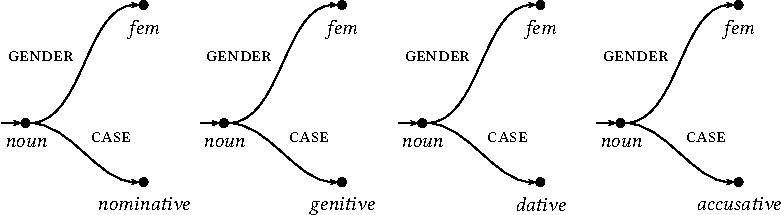
\includegraphics{Figures/frau-model-theoretic-cropped}
}
%%   \begin{pspicture}(-0.5,0.4)(2.8,4.1)
%% %\psgrid
%%      \psset{fillstyle=solid, fillcolor=black,radius=0.75mm}
%%      \pnode(-0.4,2){start1}
%%      \Cnode(0,2){noun1}
%%      \Cnode(2,4){fem1}
%%      \Cnode(2,1){nom1}
%% %
%%      \psset{fillstyle=none,nodesep=0pt,angleB=180,arrows=->} 
%% %
%%      \nccurve{start1}{noun1}
%%      \nccurve{noun1}{fem1}\naput{\textsc{gender}}
%%      \nccurve{noun1}{nom1}\naput{\textsc{case}}
%% %
%%      \nput{270}{noun1}{\type{noun}}
%%      \nput{270}{fem1}{\type{fem}}
%%      \nput{270}{nom1}{\type{nominative}}
%% \end{pspicture}
%% \begin{pspicture}(-0.5,0.4)(2.8,4.1)
%% %\psgrid
%% %
%%      \psset{fillstyle=solid, fillcolor=black,radius=0.75mm}
%%      \pnode(-0.4,2){start2}
%%      \Cnode(0,2){noun2}
%%      \Cnode(2,4){fem2}
%%      \Cnode(2,1){nom2}
%% %
%%      \psset{fillstyle=none,nodesep=0pt,angleB=180,arrows=->} 
%% %
%%      \nccurve{start2}{noun2}
%%      \nccurve{noun2}{fem2}\naput{\textsc{gender}}
%%      \nccurve{noun2}{nom2}\naput{~\textsc{case}}

%%      \nput{270}{noun2}{\type{noun}}
%%      \nput{270}{fem2}{\type{fem}}
%%      \nput{270}{nom2}{\type{genitive}}
%% \end{pspicture}
%% \begin{pspicture}(-0.5,0.4)(2.8,4.1)
%% %\psgrid
%%      \psset{fillstyle=solid, fillcolor=black,radius=0.75mm}
%%      \pnode(-0.4,2){start3}
%%      \Cnode(0,2){noun3}
%%      \Cnode(2,4){fem3}
%%      \Cnode(2,1){nom3}
%% %
%%      \psset{fillstyle=none,nodesep=0pt,angleB=180,arrows=->} 
%% %
%%      \nccurve{start3}{noun3}
%%      \nccurve{noun3}{fem3}\naput{\textsc{gender}}
%%      \nccurve{noun3}{nom3}\naput{\textsc{case}}
%% %
%%      \nput{270}{noun3}{\type{noun}}
%%      \nput{270}{fem3}{\type{fem}}
%%      \nput{270}{nom3}{\type{dative}}
%% \end{pspicture}
%% \begin{pspicture}(-0.5,0.4)(2.8,4.1)
%% %\psgrid
%%      \psset{fillstyle=solid, fillcolor=black,radius=0.75mm}
%%      \pnode(-0.4,2){start2}
%%      \Cnode(0,2){noun2}
%%      \Cnode(2,4){fem2}
%%      \Cnode(2,1){nom2}
%% %
%%      \psset{fillstyle=none,nodesep=0pt,angleB=180,arrows=->} 
%% %
%%      \nccurve{start2}{noun2}
%%      \nccurve{noun2}{fem2}\naput{\textsc{gender}}
%%      \nccurve{noun2}{nom2}\naput{\textsc{case}}
%% %
%%      \nput{270}{noun2}{\type{noun}}
%%      \nput{270}{fem2}{\type{fem}}
%%      \nput{270}{nom2}{\type{accusative}}
%% \end{pspicture}}
\caption{\label{abb-avm-frau}(\ref{avm-frau})中的Frau(女人)的特征结构描写}
%\caption{\label{abb-avm-frau}Feature structures for the description of \emph{Frau} `woman' in (\ref{avm-frau})}
\end{figure}%
%-----------------------------------------------------------------------------
\begin{figure}
%\oneline{%
\centerline{%
%% \begin{pspicture}(-0.5,0.4)(2.8,4.1)
%% %\psgrid
%% %
%% %
%%      \psset{fillstyle=solid, fillcolor=black,radius=0.75mm}
%%      \pnode(-0.4,2){start1}
%%      \Cnode(0,2){noun1}
%%      \Cnode(2,4){mas1}
%%      \Cnode(2,1){nom1}
%% %
%% %
%%      \psset{fillstyle=none,nodesep=0pt,angleB=180,arrows=->} 
%% %
%%      \nccurve{start1}{noun1}
%%      \nccurve{noun1}{mas1}\naput{\textsc{gender}}
%%      \nccurve{noun1}{nom1}\naput{\textsc{case}}
%% %
%%      \nput{270}{noun1}{\type{noun}}
%%      \nput{270}{mas1}{\type{mas}}
%%      \nput{270}{nom1}{\type{nominative}}
%% \end{pspicture}
%% \begin{pspicture}(-0.5,0.4)(2.8,4.1)
%% %\psgrid
%% %
%%      \psset{fillstyle=solid, fillcolor=black,radius=0.75mm}
%%      \pnode(-0.4,2){start2}
%%      \Cnode(0,2){noun2}
%%      \Cnode(2,4){mas2}
%%      \Cnode(2,1){nom2}
%% %
%% %
%%      \psset{fillstyle=none,nodesep=0pt,angleB=180,arrows=->} 
%% %
%%      \nccurve{start2}{noun2}
%%      \nccurve{noun2}{mas2}\naput{\textsc{gender}}
%%      \nccurve{noun2}{nom2}\naput{\textsc{case}}
%% %
%%      \nput{270}{noun2}{\type{noun}}
%%      \nput{270}{mas2}{\type{mas}}
%%      \nput{270}{nom2}{\type{dative}}
%% \end{pspicture}
%% \begin{pspicture}(-0.5,0.4)(2.8,4.1)
%% %\psgrid
%% %
%%      \psset{fillstyle=solid, fillcolor=black,radius=0.75mm}
%%      \pnode(-0.4,2){start2}
%%      \Cnode(0,2){noun2}
%%      \Cnode(2,4){mas2}
%%      \Cnode(2,1){nom2}
%% %
%% %
%%      \psset{fillstyle=none,nodesep=0pt,angleB=180,arrows=->} 
%% %
%%      \nccurve{start2}{noun2}
%%      \nccurve{noun2}{mas2}\naput{\textsc{gender}}
%%      \nccurve{noun2}{nom2}\naput{\textsc{case}}
%% %
%%      \nput{270}{noun2}{\type{noun}}
%%      \nput{270}{mas2}{\type{mas}}
%%      \nput{270}{nom2}{\type{accusative}}
%% \end{pspicture}
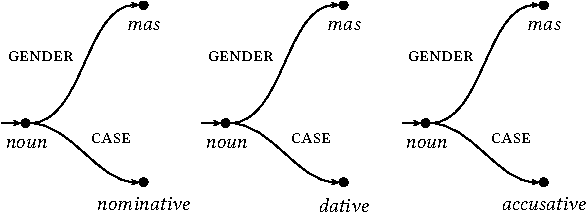
\includegraphics{Figures/mann-model-theoretic-crop}
}
\caption{\label{abb-avm-mann}(\ref{avm-mann})中的Mann(男人)的特征结构描写}
%\caption{\label{abb-avm-mann}Feature structures for the description of \emph{Mann} `man' in  (\ref{avm-mann})}
\end{figure}%
在这些表达式中,每个结点都有一定的类型(\type{名词}、\type{阴性}、\type{主格} \ldots),并且特征结构中的类型总是最具体的,即它们没有深层的次类型。总有一个入口结点(上例中的\type{名词})和其他用特征标签标注的用箭头连接起来的结点(“\textsc{性别}”、“\textsc{格}”)。
%In these representations, each node has a certain type (\type{noun}, \type{fem}, \type{nominative},
%\ldots) and the types in feature structures are always maximally specific, that is, they do not have
%any further subtypes. There is always an entry node (\type{noun} in the example above) and the other
%nodes are connected with arrows that are annotated with the feature labels (\textsc{gender}, \textsc{case}).

如果我们回到上面章节中人的例子,我们可以发现模型与描写之间的差异,如下所示:如果我们有一个人的模型,它包括名、姓、出生日期、性别和发色,那么它自然得到的结果是我们模拟的每个对象都会有生日。但是,如果这些信息在表示约束或构成搜索时没有发挥重要的作用时,我们可以在描写中省略这些细节。
%If we return to the example with people from the previous sections, we can capture the difference between a model and a description as %follows:
%if we have a model of people that includes first name, last name, date of birth, gender and hair color, then it follows that every object we %model also has a birthday.
%We can, however, decide to omit these details from our descriptions if they do not play a role for
%stating constraints or formulating searches.

语言现象、模型和形式化理论之间的联系如图\vref{abb-modell}所示。
%The connection between linguistic phenomena, the model and the formal theory is shown in Figure~\vref{abb-modell}.
\begin{figure}
\centerline{%
%{
%% \begin{pspicture}(0,0)(9.4,4.2)
%% %\psgrid
%% \rput[Bl](0,0){%
%% \begin{tabular}[b]{@{}ccc@{}}
%% phenomenon && model\\
%% \rnode{phen}{\fbox{\begin{tabular}{c}
%% linguistic\\
%% objects\\
%% \end{tabular}}}&&\rnode{modell}{\fbox{\begin{tabular}{c}
%% feature\\
%% structures\\
%% \end{tabular}}}\\[10ex]
%% &\rnode{theorie}{\fbox{\begin{tabular}{c}
%% feature\\
%% descriptions\\
%% \end{tabular}}}\\
%% &formal theory\\
%% \end{tabular}}
%% %\anodeconnect[l]{modell}[r]{phen}%
%% \ncline{->}{modell}{phen}\nbput{models}
%% %\ncdiag[angleA=180,angleB=45]{->}{modell}{theorie}
%% \psline{<-}(5.4,1.6)(6,2.4)
%% \rput[Bl](6,2){licensed by the theory} % früher Erfüllung, jetzt FR Änderung
%% \psline{->}(5,1.7)(5.6,2.4)
%% \rput[Bl](3.4,2.0){determines}
%% %\nccurve{<-}{modell}{theorie}\nbput{legt fest}
%% \ncline{->}{theorie}{phen}\naput{predicts}%
%% %\aanodeconnect[b]{modell}[tr]{theorie}%
%% %\anodeconnect[tl]{theorie}[b]{phen}%
%\end{pspicture}
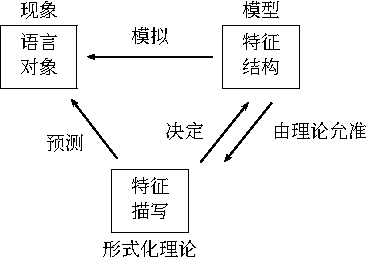
\includegraphics{Figures/model-theory-phenomenon-crop}
}
\caption{\label{abb-modell}现象、模型和形式化理论}
%\caption{\label{abb-modell}Phenomenon, model and formal theory}
\end{figure}%
\nocite{Netter98a}%S. 26
%\NOTE{WS: zwischen Modell und Theorie sollten zwei Pfeile sein.}
% ###########
% zwei Pfeile: Beschreibung legt Modell fest, um Rekursion zu erfassen (beschreibt geht wohl auch, ist aber sloppy)
%
% Modell wird von der formalen Theorie lizenziert. 
%
% Phänomen + Modell -> PS: modelliert -> lassen wir so.
%
模型是用来模拟语言现象的。进而,它必须由我们的理论所允准。理论决定了模型并且对可能的现象进行预测。
%The model is designed to model linguistic phenomena. Furthermore, it must be licensed by our theory.
%The theory determines the model and makes predictions with regard to possible phenomena.
\isce[|)]{模型}{model}\isce[|)]{理论}{theory}\isce[|)]{现象}{phenomenon}\isce[|)]{特征描写}{feature description}\isce[|)]{特征结构}{feature structure}

%\section*{思考题}
%\section*{Comprehension questions}

%\bigskip
\questions{
\begin{enumerate}
\item 使用类型的原因是什么?
\item 什么是承继?多重承继有何特殊之处?
\item 下面的结构是相容的吗?也就是说,他们能用来描写相同的对象吗?
%\item What are the reasons for using types?
%\item What is inheritance? What is special about multiple inheritance?
%\item Are the following structures compatible, that is, can they be used to describe the same object? 
\ea
\onems{
名 \type{max}\\
姓  \type{meier}\\
父亲    \ms[人]{
              名  & peter\\
              姓  & meier
             }
}\hspace{0.5cm}\onems{
名  \type{max}\\
姓  \type{meier}\\
父亲   \ms[人]{
              名  & peter\\
             姓  & müller
             }
}
\z
\ea
\onems{
名   \type{max}\\
姓   \type{meier}\\
父亲     \ms[人]{
              名 & peter\\
              姓  & meier
             }
}\hspace{0.5cm}\onems{
名   \type{max}\\
姓   \type{meier}\\
母亲      \ms[人]{
              名  & ursula\\
              姓  & müller
             }
}
\z

\end{enumerate}
}

%\section*{练习题}
%\section*{Exercises}

\exercises{
\begin{enumerate}
\item 请设想如何通过特征描写来描写乐器。
%\item Think about how one could describe musical instruments using feature descriptions.
\item 请设计一个词类(\type{限定词}、\type{标句词}、\type{名词}、\type{动词}、\type{形容词}、\type{介词})的类型层级体系。请设想可以组织类型层级的方式,这样我们可以对第\pageref{Tabelle-Merkmalszerlegung-Wortarten}页的图\ref{Tabelle-Merkmalszerlegung-Wortarten}中的二元特征的概括进行表示。
%\item Come up with a type hierarchy for the word classes (\type{det}, \type{comp}, \type{noun}, \type{verb},
%      \type{adj}, \type{prep}). Think about the ways in which one can organize the type hierachy so that one
%	  can express the generalizations that where captured by the binary features in Table~\ref{Tabelle-Merkmalszerlegung-Wortarten} on page~%\pageref{Tabelle-Merkmalszerlegung-Wortarten}.
\item\label{ua-liste}在本章,我们介绍了列表。这看起来好像是形式化的扩展,但是它并不是,因为可以将列表标记转化为只需要特征-值偶对的标记。请思考如何做到这一点。
%\item\label{ua-liste} In this chapter, we introduced lists. This may look like an extension of the formalism, but it is not as it is possible to
%convert the list notation into a notation which only requires feature-value pairs. Think about how one could do this.
\item (附加练习)附加关系(append)\iscesub{关系}{relation}{附加关系}{\emph{append}}
  将在第\ref{Kapitel-HPSG}章发挥作用。该关系用来将两个列表组合成第三个列表。诸如附加(append)的关系约束实际上构成了形式化的一种扩展。使用关系约束可以将任意数量的特征值与其他值联系起来,即我们可以写出这样的程序,它根据其他值计算出具体的值。这就导致了一个问题,在语言学理论中我们是否需要如此强有力的描写工具,并且如果我们允许使用它们,我们将会承担什么样的复杂度的代价。可见,我们最好选择那些不需要关系约束的理论,而不是那些需要关系约束的理论(参见\citet[\S~20]{MuellerLehrbuch1}对相关理论的比较)。
%\item (Additional exercise) The relation \emph{append}\is{relation!\emph{append}} will play a role in Chapter~\ref{Kapitel-HPSG}. This relation %serves to
%combine two lists to form a third.
%Relational constraints such as \emph{append} do in fact constitute an expansion of the formalism. Using relational constraints, it is possible to %relate any number
%of feature values to other values, that is, one can write programs which compute a particular value depending on other values. 
%This poses the question as to whether one needs such powerful descriptive tools in a linguistic theory and if we do allow them, what kind of %complexity we afford them.
%A theory which can do without relational constraints should be preferred over one that uses
%relational constraints (see \citealp[Chapter~20]{MuellerLehrbuch1} for a comparison of theories).

列表的串联可以在没有关系约束要求的特征结构中实现。请问这是如何做到的,并提供你的数据来源,记录下你找到解决方案的途径。
%For the concatenation of lists, there is a possible implementation in feature structures without
%recourse to relational constraints. Find out how this can be done. Give your sources and document
%how you went about finding the solution.

\end{enumerate}
}

%\section*{延伸阅读}
%\section*{Further reading}
\furtherreading{
本章为读者设计了简单易懂的有关类型特征结构的介绍。结构的数学属性、类型层级体系以及这些结构的组合性概率没有在这里进行详细说明,但是至少这些属性的一部分对于计算语言学的工作以及开发个人自己的分析来说都是非常重要的。更多的内容,我推荐感兴趣的读者阅读以下文献:
%This chapter was designed to give the reader an easy-to-follow introduction to typed feature structures. The mathematical properties of the %structures, type hierarchies and the
%combinatorial possibilities of such structures could not be discussed in detail here, but knowledge of
%at least part of these properties is important for work in computational linguistics and in
%developing one's own analyses. For more information, I refer the interested reader to the following publications: 
%
 \citet{Shieber86a}是对合一语法理论的简短介绍。它针对重要的语法类型给出了相对全面的综述,如DCG\isce{定子句文法}{Definite Clause Grammar (DCG)}、\lfgc、\gpsgc、HPSG、PATR-II\isce{PATR-II}{PATR-II}。
% \citet{Shieber86a} is a short introduction to the theory of Unification Grammar. It offers a relatively general overview followed by the %discussion of important grammar types
%such as DCG\is{Definite Clause Grammar (DCG)}, \lfg, \gpsg,
%HPSG, PATR-II\is{PATR-II}.
%
 \citet{Johnson88}按照数学的精确形式描述了非类型特征结构的形式化。
% \citet{Johnson88} describes the formalism of untyped feature structures in a mathematically precise way.
%
 \citet{Carpenter92a}重点分析了类型特征结构在数学上的表示。由 \citet{King99a-u}开发的HPSG-语法构成了 \citet{Richter2004a-u}的形式化的基础,该语法目前被看作是HPSG的标准形式化语法。
% \citet{Carpenter92a} goes into the detail about the mathematical aspects of typed feature structures. The formalism developed by 
% \citet{King99a-u} for HPSG-grammars forms the basis
%for the formalism by  \citet{Richter2004a-u}, which currently counts as the standard formalism for HPSG.
}


% lulu/wsun/sisi: DONE
%      <!-- Local IspellDict: en_US-w_accents -->
